\documentclass[hyperref, a4paper]{ctexart}
\usepackage{lmodern}
\usepackage{amssymb,amsmath}
\usepackage{ifxetex,ifluatex}
\usepackage{fixltx2e} % provides \textsubscript
\ifnum 0\ifxetex 1\fi\ifluatex 1\fi=0 % if pdftex
  \usepackage[T1]{fontenc}
  \usepackage[utf8]{inputenc}
\else % if luatex or xelatex
  \ifxetex
    \usepackage{xltxtra,xunicode}
  \else
    \usepackage{fontspec}
  \fi
  \defaultfontfeatures{Mapping=tex-text,Scale=MatchLowercase}
  \newcommand{\euro}{€}
\fi
% use upquote if available, for straight quotes in verbatim environments
\IfFileExists{upquote.sty}{\usepackage{upquote}}{}
% use microtype if available
\IfFileExists{microtype.sty}{%
\usepackage{microtype}
\UseMicrotypeSet[protrusion]{basicmath} % disable protrusion for tt fonts
}{}
\ifxetex
  \usepackage[setpagesize=false, % page size defined by xetex
              unicode=false, % unicode breaks when used with xetex
              xetex]{hyperref}
\else
  \usepackage[unicode=true]{hyperref}
\fi
\usepackage[usenames,dvipsnames]{color}
\hypersetup{breaklinks=true,
            bookmarks=true,
            pdfauthor={Tian, Jiahe; Hu, Xiaoxiao; Huang, Jiani; Liu, Jiaxing; Shi, Ruixin; Wu, Chenning; Zhang, Cenyuan; Zhang, Yihan; Wang, Chen},
            pdftitle={ 出题系统需求文档},
            colorlinks=true,
            citecolor=blue,
            urlcolor=blue,
            linkcolor=magenta,
            pdfborder={0 0 0}}
\urlstyle{same}  % don't use monospace font for urls
\setlength{\emergencystretch}{3em}  % prevent overfull lines
\providecommand{\tightlist}{%
  \setlength{\itemsep}{0pt}\setlength{\parskip}{0pt}}
\setcounter{secnumdepth}{5}

\title{\vspace{2in} 出题系统需求文档\\\vspace{0.5em}{\large 软件质量保障与测试课程Lab1课程作业(第9组)}}
\author{Tian, Jiahe\footnote{Equal Contribution, Fudan University, 17307130313
  (\href{mailto:tianjh17@fudan.edu.cn}{\nolinkurl{tianjh17@fudan.edu.cn}})} \and Hu, Xiaoxiao\footnote{Equal Contribution, Fudan University, 17302010077
  (\href{mailto:xxhu17@fudan.edu.cn}{\nolinkurl{xxhu17@fudan.edu.cn}})} \and Huang, Jiani\footnote{Equal Contribution, Fudan University, 17302010063
  (\href{mailto:huangjn17@fudan.edu.cn}{\nolinkurl{huangjn17@fudan.edu.cn}})} \and Liu, Jiaxing\footnote{Equal Contribution, Fudan University, 17302010049
  (\href{mailto:jiaxingliu17@fudan.edu.cn}{\nolinkurl{jiaxingliu17@fudan.edu.cn}})} \and Shi, Ruixin\footnote{Equal Contribution, Fudan University, 17302010065
  (\href{mailto:rxshi17@fudan.edu.cn}{\nolinkurl{rxshi17@fudan.edu.cn}})} \and Wu, Chenning\footnote{Equal Contribution, Fudan University, 17302010066
  (\href{mailto:cnwu17@fudan.edu.cn}{\nolinkurl{cnwu17@fudan.edu.cn}})} \and Zhang, Cenyuan\footnote{Equal Contribution, Fudan University,
  17302010068
  (\href{mailto:cenyuanzhang17@fudan.edu.cn}{\nolinkurl{cenyuanzhang17@fudan.edu.cn}})} \and Zhang, Yihan\footnote{Equal Contribution, Fudan University, 17302010076
  (\href{mailto:zhangyihan17@fudan.edu.cn}{\nolinkurl{zhangyihan17@fudan.edu.cn}})} \and Wang, Chen\footnote{Equal Contribution, Fudan University, 16307110064
  (\href{mailto:wangc16@fudan.edu.cn}{\nolinkurl{wangc16@fudan.edu.cn}})}}
\date{2020年3月12日}



% Redefines (sub)paragraphs to behave more like sections
\ifx\paragraph\undefined\else
\let\oldparagraph\paragraph
\renewcommand{\paragraph}[1]{\oldparagraph{#1}\mbox{}}
\fi
\ifx\subparagraph\undefined\else
\let\oldsubparagraph\subparagraph
\renewcommand{\subparagraph}[1]{\oldsubparagraph{#1}\mbox{}}
\fi

\begin{document}
\maketitle

\newpage

\LARGE

\begin{center}
\textbf{出题系统需求文档}
\end{center}

\large
\begin{center}
\textbf{\emph{软件质量保障与测试课程Lab1课程作业}}
\end{center}

\hypertarget{ux6458ux8981}{%
\section*{摘要}\label{ux6458ux8981}}
\addcontentsline{toc}{section}{摘要}

本次作业为软件质量保障与测试课程的Lab1课程作业,需要我们以小组为单位阅读、理解出题系统初始需求文档,进行小组讨论,结合软件质量相关属性,提出潜在存在的需求重构点,并自定义需求规范撰写需求文档,结合``禅道''平台辅助进行需求管理。

\hypertarget{ux5173ux952eux8bcd}{%
\section*{关键词}\label{ux5173ux952eux8bcd}}
\addcontentsline{toc}{section}{关键词}

系统与软件工程; 系统与软件质量要求和评价; 需求文档

\hypertarget{ux7248ux672cux5386ux53f2}{%
\section*{版本历史}\label{ux7248ux672cux5386ux53f2}}
\addcontentsline{toc}{section}{版本历史}

\begin{center}
%干我的居中失败了why
\begin{tabular}{|p{2cm}|p{3.3cm}|p{8cm}|}
\hline
版本 & 日期 & 说明\\
\hline
草稿 & 2014 年2 月6 日 & 建立此文档\\
\hline
Alpha 版 & 2014 年2 月8 日 & 做了修改后进行内部评审\\
\hline
Alpha 03 & 2014 年2 月9 日 & 魏X 内部评审稿\\
\hline
Alpha 04 & 2014 年2 月11 日 & 黄X 增加属性,完善评审流程\\
\hline
Alpha 05 & 2014 年2 月14 日 & 增加周X 的问题\\
\hline
Alpha 06 & 2014 年2 月17 日 & 增加T 模块考卷规则、增加分值规则\\
\hline
发布版 1.0 & 2014 年3 月10 日 & 修改后发布\\
\hline
发布版 2.0 & 2014 年3 月16 日 & 评审后,经修改后发布\\
\hline
修订版3.1 & 2014 年4 月25 日 & 与开发商和办公室讨论后收集的建议和问题\\
\hline
修订版3.2 & 2014 年5 月21 日 & 回答魏X 的问题\\
\hline
修订版3.3 & 2014 年6 月30 日 & 根据开发商反馈建议和需求细化后整理。\\
\hline
发布版3.0 & 2014 年7 月1 日 & 修改后发布。所有状态的描述重新编写,更加便于理解。加入新的考题属性“理论实践”。部分修改和完善。\\
\hline
修订版4.0 & 2020 年3 月12 日 & 进行合理性检查和规范定义后整理。\\
\hline
\end{tabular}
\end{center}

\normalsize

\newpage

\tableofcontents

\newpage

\hypertarget{ux5728ux7ebfux51faux9898ux8003ux8bd5ux7cfbux7edfux6982ux8ff0ux5b8cux6574ux7cfbux7edf}{%
\section*{在线出题考试系统概述(完整系统)}\label{ux5728ux7ebfux51faux9898ux8003ux8bd5ux7cfbux7edfux6982ux8ff0ux5b8cux6574ux7cfbux7edf}}
\addcontentsline{toc}{section}{在线出题考试系统概述(完整系统)}

``在线出题考试系统''是为组织考试的一个基于Web
的在线系统,主要由``出题系统''、``题库管理系统''、``在线报名和考生管理系统''以及``考试系统''四大模块(子系统)组成。

\hypertarget{ux51faux9898ux7cfbux7edfux63cfux8ff0}{%
\section*{出题系统描述}\label{ux51faux9898ux7cfbux7edfux63cfux8ff0}}
\addcontentsline{toc}{section}{出题系统描述}

出题系统是在线出题考试系统的的一个子系统。利用出题系统,出题专家们可以方便的进行网上考题编写和评审,并无缝的与在线出题考试系统进行衔接,提高考题编写的质量和效率,也便于考题的统一管理和评估。
在出题系统中,每一次的出题活动定义为一个``项目''(Project),每个项目有它的目的、内容、角色(成员)、时间(限期)和结果(输出)。例如:某一个项目可能要求出一份或几份完整的,有若干考题组成的完整``考卷'',也有可能是针对某一个或某几个``知识点''编写相应考题。在一个项目中定义了一系列``角色'',如项目的``主持人''、编写考题的``作者''和考题的``评审员''以及最后对考题把关的``质管员''等。
在出题系统中的最小单元是``考题'',``考题''包括了``考题信息''和``考题属性(辅助信息)'',``考题信息''又有``场景描述''(可有可无)、``题干''和``选项''组成;而``辅助信息''是指``考题''在它的整个生命周期中,在管理、统计、评估和自动出考卷过程所使用的一些辅助元素,在这里称为考题的``属性'',包括此考题覆盖大纲的``章节''、``知识点''和``K级(Kn)''、``状态''、``作者''、``评审员''、``质管员''、``发布时间(启用时间)''、``使用次数(使用频率)''、``答对率(每次累加)''、``答错率(每次累加)''、``出题难度(作者的预估)''、``反馈难度(学生反馈)''等(可参看考题属性描述)。这些考题经编写、评审并通过审核后可以``发布'',并以统一的格式导出和存放到题库管理系统。

\hypertarget{ux5b9aux4e49}{%
\section{定义}\label{ux5b9aux4e49}}

\hypertarget{ux57faux672cux5b9aux4e49}{%
\subsection{基本定义}\label{ux57faux672cux5b9aux4e49}}

\hypertarget{ux8003ux5377}{%
\subsubsection{考卷}\label{ux8003ux5377}}

考卷是由若干考题组成,并按照出题规则,主要根据考卷相对应大纲的知识点(对应大纲的章/节)以及知识点的K级,可参看考卷组成规则。

\hypertarget{ux8003ux9898}{%
\subsubsection{考题}\label{ux8003ux9898}}

考题是组成考卷的最小单位,由属于考题本身的考题信息以及为管理考题所需的考题属性组成。考题信息又包括该考题场景、考题题干和考题选项。考题属性包含对考题管理所需的各种属性,如考题的作者、考题的ID、考题评审者、考题的状态等,可参看考题属性表。

\hypertarget{ux77e5ux8bc6ux70b9}{%
\subsubsection{知识点}\label{ux77e5ux8bc6ux70b9}}

考题根据大纲所覆盖的章节内容,是出题的依据和范围。且每个知识点有其对应的K级别。

\hypertarget{ux6b63ux786eux9009ux9879}{%
\subsubsection{正确选项}\label{ux6b63ux786eux9009ux9879}}

考题可以是正选题,例如在考题中选择哪项是正确的,也可以是反选题,例如在考题中要求选择哪个是错误或不正确的,无论是正选还是反选题,如果考生做了正确的选择,那个被选中的选项定义为正确的选项。

\hypertarget{ux51faux9898ux7cfbux7edfux89d2ux8272}{%
\subsection{出题系统角色:}\label{ux51faux9898ux7cfbux7edfux89d2ux8272}}

\hypertarget{ux7cfbux7edfux7ba1ux7406ux5458}{%
\subsubsection{系统管理员}\label{ux7cfbux7edfux7ba1ux7406ux5458}}

负责该系统中所有用户账户的开设,创建新项目(项目名+主持人);对整个系统的配置
和运行负责;维护系统和系统数据(如大纲知识点的更新等)。

\hypertarget{ux4e3bux6301ux4eba}{%
\subsubsection{主持人}\label{ux4e3bux6301ux4eba}}

整个考题的编写和评审流程的发起人和负责人。指定此次考题对应的大纲知识点,将考
题分配给指定的作者、评审员和质管员,设定考题编写和评审时限。可以导出质管员同
意发布的考题。每题考题的评审员可以有多人。

\hypertarget{ux4f5cux8005}{%
\subsubsection{作者}\label{ux4f5cux8005}}

考题的编写者,收到由主持人指定需要出的考题对应的大纲知识点等信息后开始编写考
题,也可根据评审员的意见修改考题。

\hypertarget{ux8bc4ux5ba1ux5458}{%
\subsubsection{评审员}\label{ux8bc4ux5ba1ux5458}}

可对由主持人分配的,并由对应作者已编写的考题进行评审,提出评审和修改意见。

\hypertarget{ux8d28ux7ba1ux5458}{%
\subsubsection{质管员}\label{ux8d28ux7ba1ux5458}}

是最后保障考题质量的把关和负责人,由主持人指定考题的质管员,在考题通过评审后
进入``再审''状态,在``再审''状态下质管员决定是否需要返回给作者修改或者直接发布或者作废。

\hypertarget{ux8003ux9898ux7684ux72b6ux6001}{%
\subsection{考题的状态}\label{ux8003ux9898ux7684ux72b6ux6001}}

\hypertarget{ux5f00ux59cbux72b6ux6001}{%
\subsubsection{开始状态}\label{ux5f00ux59cbux72b6ux6001}}

由主持人创建一个新的考题(考题的ID),新创建考题的状态为``开始''。主持人在开始
状态为考题建立框架,分配考题对应的知识点、时间安排、分配作者和评审员以及质管
员等,完成相关设定后主持人将考题的状态从``开始''改为``编写''状态。

\hypertarget{ux7f16ux5199ux72b6ux6001}{%
\subsubsection{编写状态}\label{ux7f16ux5199ux72b6ux6001}}

在``编写''状态下,作者根据被指定的章节知识点来编写考题信息内容(场景,题干,选项),作者填写必须或应该填写的考题属性内容。作者编写考题完毕后,作者将此考题的状态从``编写''改写为``评审''状态。

\hypertarget{ux8bc4ux5ba1ux72b6ux6001}{%
\subsubsection{评审状态}\label{ux8bc4ux5ba1ux72b6ux6001}}

在``评审''状态下,评审员对作者编写或修改的考题进行评审,每一考题的评审员由主持人事先指定。评审员完成评审活动后,根据评审结果评审员可将此考题的状态从``评审''改写为``再审''或``修改''状态。例如,评审结果为``可接受''或``被拒绝'',则评审员将此考题的状态从``评审''改写为``再审''状态。如果评审结果为``需修改'',则评审员将此考题的状态从``评审''改写为``修改''状态。

\hypertarget{ux518dux5ba1ux72b6ux6001}{%
\subsubsection{再审状态}\label{ux518dux5ba1ux72b6ux6001}}

当考题处于``再审''状态,质管员对考题质量进行再次审核。根据再审结果,质管员可以将此考题的状态从``再审''改为``修改''、``发布''或``作废''状态。
\emph{备注:评审员或质管员应该在规定时限内完成评审活动并提交评审意见,如果超出规定时限评审员没有完成评审,系统自动向相关评审员或质管员发出提示信息(Mail),并同时向主持人发出信息(Mail),收到信息后主持人根据实际情况重新进行调整,可通过多重渠道进行调整:延长时间、重新安排评审员或质管员、直至删除该题等。}

\hypertarget{ux4feeux6539ux72b6ux6001}{%
\subsubsection{修改状态}\label{ux4feeux6539ux72b6ux6001}}

当考题处于``修改''状态时,考题的作者可以对考题进行修改,作者一般是参照评审的
记录和要求对考题进行修改。修改完毕后,作者可将此题的状态从``修改''改为``评审''
状态。

\hypertarget{ux53d1ux5e03ux72b6ux6001}{%
\subsubsection{发布状态}\label{ux53d1ux5e03ux72b6ux6001}}

当考题处于``发布''状态时,表示此题已经通过编写和评审,可以被使用了。主持人可
以导出此状态下的考题。主持人可以单题导出,也可以批量导出。

\hypertarget{ux4f5cux5e9fux72b6ux6001}{%
\subsubsection{作废状态}\label{ux4f5cux5e9fux72b6ux6001}}

当考题处于``作废''状态时,表示此题由于各种原因不被接受,也不会使用,主持人对
此类考题按照规定进行处理,例如删除。

\hypertarget{ux529fux80fdux6027ux9700ux6c42}{%
\section{功能性需求}\label{ux529fux80fdux6027ux9700ux6c42}}

\hypertarget{ux767bux9646ux53caux4e2aux4ebaux4fe1ux606f}{%
\subsection{登陆及个人信息}\label{ux767bux9646ux53caux4e2aux4ebaux4fe1ux606f}}

未登录状态下,用户输入正确的用户名和密码,进入登录状态,获得系统使用权限。登录状态下,用户可以修改个人信息。

\hypertarget{ux767bux5f55ux6821ux9a8c}{%
\subsubsection{登录校验}\label{ux767bux5f55ux6821ux9a8c}}

\begin{itemize}
\tightlist
\item
  关键词:登录~匹配
\item
  在用户属于未登录状态下,用户输入正确的用户名和密码,进入登录状态,可以根据用户权限对考题进行创建、修改或评审。用户输入错误的用户名或密码,提示``用户名或密码''错误,允许继续输入,不允许对考题进行任一操作。
\item
  验收标准:用户能够正确登录系统,登录状态由``未登录''变为对应用户名。
\end{itemize}

\hypertarget{ux4feeux6539ux4e2aux4ebaux4fe1ux606f}{%
\subsubsection{修改个人信息}\label{ux4feeux6539ux4e2aux4ebaux4fe1ux606f}}

\begin{itemize}
\tightlist
\item
  关键词:个人信息~修改
\item
  在用户处于登录状态下,可以对用户信息(包括用户名、密码、其他信息等)进行修改。修改完成后自动更新用户信息。
\item
  验收标准:用户能够完成信息修改并正确显示。
\end{itemize}

\hypertarget{ux5efaux7acbux65b0ux9879ux76ee}{%
\subsection{建立新项目}\label{ux5efaux7acbux65b0ux9879ux76ee}}

完成登录后,主持人需要创建新的项目,并对其进行规划。项目创建完成后,主持人需要在其中创建新的题目并设置题目属性、分配作者与评审员。

\hypertarget{ux521bux5efaux9879ux76ee}{%
\subsubsection{创建项目}\label{ux521bux5efaux9879ux76ee}}

\begin{itemize}
\tightlist
\item
  关键词:新建~系统~主持人
\item
  主持人创建新的出题系统,不允许更换其他主持人。在创建时定义项目名,不能与其他出题系统重复,不允许创建完成后修改。
\item
  主持人在创建项目时可以对项目进行规划,如限制项目考题数量或考题范围。
\item
  验收标准:主持人成功创建项目,确定项目名称以及项目规划,并通过邮件提示主持人。
\end{itemize}

\hypertarget{ux65b0ux5efaux8003ux9898}{%
\subsubsection{新建考题}\label{ux65b0ux5efaux8003ux9898}}

\begin{itemize}
\tightlist
\item
  关键词:新建~考题~属性~管理人员
\item
  主持人在完成项目创建后可以创建新考题,创建时为考题确定唯一不重复ID。主持人设置考题状态为``开始'',在开始状态下为考题设置题目属性(如时间点、时间安排)。
\item
  主持人在开始状态下为考题设置相关管理人员,包括作者、评审员、质管员。其中不同身份不能安排同一名用户,如作者与评审员不能有同一个用户ID。每个身份要求至少安排一人,允许为一道考题安排多名作者、评审员、质管员。同时允许评审员和作者之间互相读取权限信息。
\item
  验收标准:主持人成功新建题目、设置题目属性与作者、评审员,并自动发送邮件给对应管理人员进行确认。
\end{itemize}

\hypertarget{ux5f00ux59cbux542fux52a8ux9879ux76eeux72b6ux6001-ux5f00ux59cb-ux89d2ux8272-ux4e3bux6301ux4eba}{%
\subsection{开始启动项目(状态: 开始; 角色:
主持人)}\label{ux5f00ux59cbux542fux52a8ux9879ux76eeux72b6ux6001-ux5f00ux59cb-ux89d2ux8272-ux4e3bux6301ux4eba}}

在开始状态下,主持人可以为题目分配知识点,设置期限与管理人员。在完成设置后允许主持人将题目状态改为``编写'',由系统自动提示作者进行编写,编写过程存在时间限制。

\hypertarget{ux8bbeux7f6eux671fux9650}{%
\subsubsection{设置期限}\label{ux8bbeux7f6eux671fux9650}}

\begin{itemize}
\tightlist
\item
  关键词:开始~期限~警告
\item
  主持人为开始状态下的考题分配知识点,设定编写考题与评审考题的时间限制。
\item
  设置完成后,当作者和评审员修改对应考题时,系统对超出时间限制的任务进行报警,自动发送邮件或站内信给主持人。主持人收到报警后可以选择对超出期限的任务提出警告或是延长时间限制。
\item
  验收标准:主持人成功设置考题编写与评审时间限制,并在超出限制时收到邮件或站内信。
\end{itemize}

\hypertarget{ux4feeux6539ux72b6ux6001ux5f00ux59cb-ux7f16ux5199}{%
\subsubsection{修改状态(开始-编写)}\label{ux4feeux6539ux72b6ux6001ux5f00ux59cb-ux7f16ux5199}}

\begin{itemize}
\tightlist
\item
  关键词:编写~作者
\item
  主持人在开始状态下完成了对题目属性的设置、知识点的分配、作者、评审员和质管员的设置后,可以将题目状态改为``编写''。系统自动向状态为``编写''题目的作者发送提示邮件。
\item
  未完成相应设置的题目不允许修改状态。允许批量修改多个题目状态。
\item
  验收标准:主持人成功修改题目状态,作者收到邮件通知。
\end{itemize}

\hypertarget{ux7f16ux5199ux8003ux9898ux72b6ux6001-ux7f16ux5199-ux89d2ux8272-ux4f5cux8005}{%
\subsection{编写考题(状态: 编写; 角色:
作者)}\label{ux7f16ux5199ux8003ux9898ux72b6ux6001-ux7f16ux5199-ux89d2ux8272-ux4f5cux8005}}

在编写状态下,作者应对多种格式的题目(包括普通文字、表格、图形)进行手动编写或限制格式的自动导入。在确保题目进行充分编写后,作者可以修改题目状态,提交评审。

\hypertarget{ux8bbeux7f6eux591aux7c7bux578bux8003ux9898}{%
\subsubsection{设置多类型考题}\label{ux8bbeux7f6eux591aux7c7bux578bux8003ux9898}}

\begin{itemize}
\tightlist
\item
  关键词:编写~答案
\item
  在编写状态下,作者可以看到由主持人分配给自己编写的考题。作者允许编写普通(纯文字)考题、带有表格或图形的考题并正确显示,无乱码。同时,作者需要对题目给出标准答案并设置相关属性(如题型、知识点、分值等)。
\item
  作者可以手动输入考题,也可以对普通考题、带有表格或图形对考题以XML,
  Excel的形式导入出题系统。
\item
  验收标准:作者正确编写或导入多种格式的考题,显示正确。
\end{itemize}

\hypertarget{ux4feeux6539ux72b6ux6001ux7f16ux5199-ux8bc4ux5ba1}{%
\subsubsection{修改状态(编写-评审)}\label{ux4feeux6539ux72b6ux6001ux7f16ux5199-ux8bc4ux5ba1}}

\begin{itemize}
\tightlist
\item
  关键词:状态~评审
\item
  在编写过程中,作者不允许对评审员、质管员进行修改,也不允许修改题目的编写时间限制或所属项目。仅允许且必须对题干、答案和部分题目属性进行编写和设置。
\item
  在完成题目、答案与属性编写后,作者需要把题目状态设置为``评审''。由系统自动发送邮件给评审员,提醒评审。未完成编写对题目不允许修改状态,仍保持``编写''状态。
\item
  验收标准:作者完成题目编写后正确修改题目状态,评审员收到邮件通知。
\end{itemize}

\hypertarget{ux8bc4ux5ba1ux8003ux9898ux72b6ux6001-ux8bc4ux5ba1-ux89d2ux8272-ux8bc4ux5ba1ux5458}{%
\subsection{评审考题(状态: 评审; 角色:
评审员)}\label{ux8bc4ux5ba1ux8003ux9898ux72b6ux6001-ux8bc4ux5ba1-ux89d2ux8272-ux8bc4ux5ba1ux5458}}

在评审状态下,评审员只能查看由主持人分配属于需要自己评审的考题,
或已经评审过但经作者修改后需要再次评审的考题,并对这些考题进行评审。

\begin{table}[!htbp]
  \caption{评审说明}
  \label{Tab:bookRWCal}
  \centering
  \begin{tabular}{|l|p{1.5cm}|p{5.3cm}|p{3.3cm}|}
  \hline
  \textbf{序号} &\textbf{评审结果} &\textbf{说明}&\textbf{备注}\\
  \hline
  01 & 可接受  & 评审中没有(再)发现考题中有错误,考题也满足了出题的要求,
  覆盖了相应的 大纲知识点。& 此题可以进行再评审,如果再评审没发现问题,则可发布。\\
  \hline
  02 & 需修改  & 评审如果(再)发现考题中有错误,或(和)考题没用满足出题的要求,
  或(和)考题没用覆盖相应的大纲知识点。& 此题可以进行再评审,如果再评审没发现问题,则可发布。\\
  \hline
  03  & 被拒绝 & 评审中发现有非常严重的错误,根本无 法修改,或不值修改。或者考题完全偏
  离了出题的要求,或者没有覆盖相应的大纲知识点。& 此题可以进行再评审,如果质量管理员也认可评审员的决定,则可作废此题。\\
  \hline
  \end{tabular}
\end{table}

\hypertarget{ux8bc4ux5ba1ux53efux63a5ux53d7}{%
\subsubsection{评审可接受}\label{ux8bc4ux5ba1ux53efux63a5ux53d7}}

\begin{itemize}
\tightlist
\item
  关键词:可接受~再审
\item
  如果评审员在评审过程中没有(再)发现考题中有错误,考题也满足了出题的要求,覆盖了
  相应的大纲知识点,则评审员设置评审结果为``可接受'',并且评审员将考题的状态从``评
  审''改为``再审''(第二次评审),系统会自动给质管员(质量管理员)发送相应的提示电邮。
\item
  验收标准:评审员能够正确设置评审结果为``可接受'',考题的状态从``评审''变为``再审'',能够通过邮件提醒相关质管员。
\end{itemize}

\hypertarget{ux8bc4ux5ba1ux88abux62d2ux7edd}{%
\subsubsection{评审被拒绝}\label{ux8bc4ux5ba1ux88abux62d2ux7edd}}

\begin{itemize}
\tightlist
\item
  关键词:被拒绝~再审
\item
  如果评审员在评审过程中发现考题有非常严重的错误,根本无法修改,或不值修改。
  或者考题完全偏离了出题的要求,或者没有覆盖相应的大纲知识点,
  则评审员设置评审结果为``被拒绝'',并且将考题的状态从``评审''修改为``再审''(第二次评审),
  系统会自动给质管员 (质量管理员)发送相应的提示电邮。
\item
  验收标准:评审员能够正确设置考题的状态从``再审''变为``发布'',能够通过邮件提醒相关质管员。
\end{itemize}

\hypertarget{ux8bc4ux5ba1ux9700ux4feeux6539}{%
\subsubsection{评审需修改}\label{ux8bc4ux5ba1ux9700ux4feeux6539}}

\begin{itemize}
\tightlist
\item
  关键词:需修改~修改
\item
  如果评审员在评审过程中发现考题中有错误,或(和)考题没有满足出题的要求,
  或(和)考题没有覆盖相应的大纲知识点,并要求作者进行修改,则评审员设置评审结果为``需修改'',
  并且将考题的状态从``评审''改为``修改'',系统会自动给作者发送相应的提示电邮。
\item
  验收标准:评审员能够正确设置评审结果为``需修改'',考题的状态从``评审''变为``修改'',能够通过邮件提醒作者。
\end{itemize}

\hypertarget{ux8bc4ux5ba1ux6743ux9650ux63a7ux5236}{%
\subsubsection{评审权限控制}\label{ux8bc4ux5ba1ux6743ux9650ux63a7ux5236}}

\begin{itemize}
\tightlist
\item
  关键词:评审员权力~主持人权力
\item
  在评审状态下,评审员有权可以阅读被主持人分配属于需要自己评审的考题,
  也有权对此考题编写评审意见和建议,或指出错误所在。评审员有权可以改变属于需要自己
  评审的考题的状态(从``评审''到``再审'',或从``评审''到``修改'')。在评审状态下主持
  人只有阅读的权限,
  没有修改(考题和属性的修改)和操作(改变状态)的权限。
\item
  验收标准:评审员可以正常行使阅读,评审和修改考题状态的权力,主持人只能阅读。
\end{itemize}

\hypertarget{ux518dux5ba1ux8003ux9898ux72b6ux6001-ux518dux5ba1-ux89d2ux8272-ux8d28ux7ba1ux5458}{%
\subsection{再审考题(状态: 再审; 角色:
质管员)}\label{ux518dux5ba1ux8003ux9898ux72b6ux6001-ux518dux5ba1-ux89d2ux8272-ux8d28ux7ba1ux5458}}

在再审状态下,质管员(质量管理员)要做最后的质量把关。在再评审过程,质量管理员可
以根据评审员的评审结果(可接受、需修改、被拒绝),
以及凭借自己的专业水平和敬业精 神对考题进行评审和把关。

\hypertarget{ux518dux5ba1ux53efux53d1ux5e03}{%
\subsubsection{再审可发布}\label{ux518dux5ba1ux53efux53d1ux5e03}}

\begin{itemize}
\tightlist
\item
  关键词:可接受~发布
\item
  如果此考题的评审结果是``可接受'',在再审过程中,
  质量管理员也认为此题确实可以发布,
  则将此题的状态从``再审''修改为``发布''。表示此题可以发布。
  系统都会自动给主持人发出提示电邮。
\item
  验收标准:评审员能够正确设置考题的状态,从``再审''变为``发布'',能够通过邮件提醒主持人。
\end{itemize}

\hypertarget{ux518dux5ba1ux9700ux4feeux6539}{%
\subsubsection{再审需修改}\label{ux518dux5ba1ux9700ux4feeux6539}}

\begin{itemize}
\tightlist
\item
  关键词:可接受~被拒绝~修改
\item
  评审结果为``可接受'',但质量管理员在再审过程中发现一些错误,
  甚至考题没有满足出题的要求,或(和)考题没有覆盖相应的大纲知识点。
  质量管理员也可要求作者进行修改,并将考题的状态从``再审''修改为``修改''。
  系统会自动给作者发送相应的提示电邮。
\item
  评审结果为``被拒绝'',但质量管理员在再审过程中发现考题基本上满足了出题的要求,或(和)考题没基本上覆盖了相应的大纲知识点,但略有不足之处。质量管理员可要求作者进行修改,并将考题的状态从``再审''修改为``修改''。系统会自动给作者发送相应的提示电邮。
\item
  验收标准:评审员能够正确设置考题的状态,从``再审''变为``修改'',能够通过邮件提醒作者。
\end{itemize}

\hypertarget{ux518dux5ba1ux9700ux4f5cux5e9f}{%
\subsubsection{再审需作废}\label{ux518dux5ba1ux9700ux4f5cux5e9f}}

\begin{itemize}
\tightlist
\item
  关键词:被拒绝~作废
\item
  如果此考题的评审结果是``被拒绝'',在再审过程中,质量管理员也认为此题确实应该作废,
  则将此题的状态从``再审''修改为``作废''。表示此题已被作废。
  系统都会自动给主持人发出提示电邮。
\item
  验收标准:评审员能够正确设置考题的状态,从``再审''变为``作废'',能够通过邮件提醒主持人。
\end{itemize}

\hypertarget{ux518dux5ba1ux6743ux9650ux63a7ux5236}{%
\subsubsection{再审权限控制}\label{ux518dux5ba1ux6743ux9650ux63a7ux5236}}

\begin{itemize}
\tightlist
\item
  关键词:质管员权力~主持人权力
\item
  在再审状态下,质管员(质量管理员)有权阅读所有处于``再审''的考题, 也
  有权对这些考题编写评审意见和建议,或指出错误所在。质管员(质量管理员)有权改变处
  于``再审''考题的状态(从``再审''到``修改'',或从``再审''到``发布'',或从``再审''到
  ``作废'')。在再审状态下主持人只有阅读的权限,
  没有修改考题(考题和属性的修改)和操 作(改变状态)的权限。
\item
  验收标准:质管员可以正常行使阅读,评审,修改考题状态的权力,主持人只能阅读。
\end{itemize}

\hypertarget{ux4feeux6539ux8003ux9898ux72b6ux6001-ux4feeux6539-ux89d2ux8272-ux4f5cux8005}{%
\subsection{修改考题(状态: 修改; 角色:
作者)}\label{ux4feeux6539ux8003ux9898ux72b6ux6001-ux4feeux6539-ux89d2ux8272-ux4f5cux8005}}

\hypertarget{ux4feeux6539ux8003ux9898}{%
\subsubsection{修改考题}\label{ux4feeux6539ux8003ux9898}}

\begin{itemize}
\tightlist
\item
  关键词:修改~评审
\item
  在修改状态下,作者可以阅读到所有与本作者有关的需要修改的考题,
  这些修改要求有可能是评审员要求的,也有可能是质量管理员在``再审''时要求的。
  作者在仔细阅读修改要求或修改意见或建议后,并参看大纲,认真思考,对考题进行修改。
  修改完毕后,作者将此题的状态从``修改''再改变为``评审'',系统会自动给评审员发出提示电邮。
\item
  验收标准:作者可以阅读修改要求、意见,并对考题进行修改。作者能够正确的是指考题状态,从修改到``评审''。
  能够通过邮件提醒相关评审员。
\end{itemize}

\hypertarget{ux4feeux6539ux6743ux9650ux63a7ux5236}{%
\subsubsection{修改权限控制}\label{ux4feeux6539ux6743ux9650ux63a7ux5236}}

\begin{itemize}
\tightlist
\item
  关键词:作者权力~主持人权力
\item
  在修改状态下,作者有权阅读所有属于需要自己修改的考题,
  有权对这些考题进行修改。作者有权改变处于``修改''考题的状态(从``修改''到``评审'')。
  在修改状态下
  主持人只有阅读的权限,没有修改(考题和属性的修改)和操作(改变状态)的权限。
\item
  验收标准:作者可以正常行使阅读,修改考题的权力,主持人只能阅读。
\end{itemize}

\hypertarget{ux53d1ux5e03ux8003ux9898ux72b6ux6001-ux53d1ux5e03-ux89d2ux8272-ux4e3bux6301ux4eba}{%
\subsection{发布考题(状态: 发布; 角色:
主持人)}\label{ux53d1ux5e03ux8003ux9898ux72b6ux6001-ux53d1ux5e03-ux89d2ux8272-ux4e3bux6301ux4eba}}

\hypertarget{ux5bfcux51faux53d1ux5e03ux8003ux9898}{%
\subsubsection{导出发布考题}\label{ux5bfcux51faux53d1ux5e03ux8003ux9898}}

\begin{itemize}
\item
  关键词:发布~导出
\item
  在考题处于``发布''状态下,主持人可以阅读所有这些已发布的考题,并且根据考题导出规则导出这些考题。主持人没有修改考题(包含考题的内容和属性)和操作(改变状态)的权限。
\item
  此处限定考题导出规则为:(以从高到低的优先级顺序排列)根据考题的发布时间、考题的id命名规则、参与该考题出题和评审的人员信息的顺序导出考题。
\item
  此处限定考题导出内容为:考题最终发布版本的所有完整内容及属性和考题的历史数据(包括评审内容、评审结果和修改内容)
\item
  验收标准:主持人能够查看并以Excel和XML的文件格式正确导出处于发布状态的考题的所有内容。
\end{itemize}

\hypertarget{ux5bfcux5165ux9898ux5e93}{%
\subsubsection{导入题库}\label{ux5bfcux5165ux9898ux5e93}}

\begin{itemize}
\item
  关键词:导入
\item
  题库系统管理员可以将已发布并且由主持人导出的考题(Excel文件和XML文件)文件导入题库系统,题库系统必须支持该两种格式的考题文件。
\item
  验收标准:题库系统管理员可以正确将考题文件导入题库系统。
\end{itemize}

\hypertarget{ux4f5cux5e9fux8003ux9898ux72b6ux6001-ux4f5cux5e9f-ux89d2ux8272-ux4e3bux6301ux4eba}{%
\subsection{作废考题(状态: 作废; 角色:
主持人)}\label{ux4f5cux5e9fux8003ux9898ux72b6ux6001-ux4f5cux5e9f-ux89d2ux8272-ux4e3bux6301ux4eba}}

\hypertarget{ux5e9fux9664ux4f5cux5e9fux8003ux9898}{%
\subsubsection{废除作废考题}\label{ux5e9fux9664ux4f5cux5e9fux8003ux9898}}

\begin{itemize}
\item
  关键词:作废~废除
\item
  主持人查看所有处于作废状态的考题,并且废除这些考题(即这些考题将永远不会被使用)。主持人不能修改考题和改变考题状态。
\item
  验收标准:主持人能够查看所有处于作废状态的考题。
\end{itemize}

\hypertarget{ux91cdux542fux51faux9898ux6d41ux7a0b}{%
\subsubsection{重启出题流程}\label{ux91cdux542fux51faux9898ux6d41ux7a0b}}

\begin{itemize}
\item
  关键词:作废~重启
\item
  主持人对于处于作废状态的考题进行判断后,发现无法达成出题目的和要求,重新启动项目,进行新考题的编写与评审。
\item
  验收标准:主持人能够根据出题目的和要求,根据作废考题的情况,重新启动项目。
\end{itemize}

\hypertarget{umlux5efaux6a21}{%
\subsection{UML建模}\label{umlux5efaux6a21}}

对于我们分析的流程,除了上面的文字描述之外,我们还以如下这些流程图的形式进行了体现。流程图中所展示的流程与上面小节的描述是一致的。

\begin{figure}
  \centering
  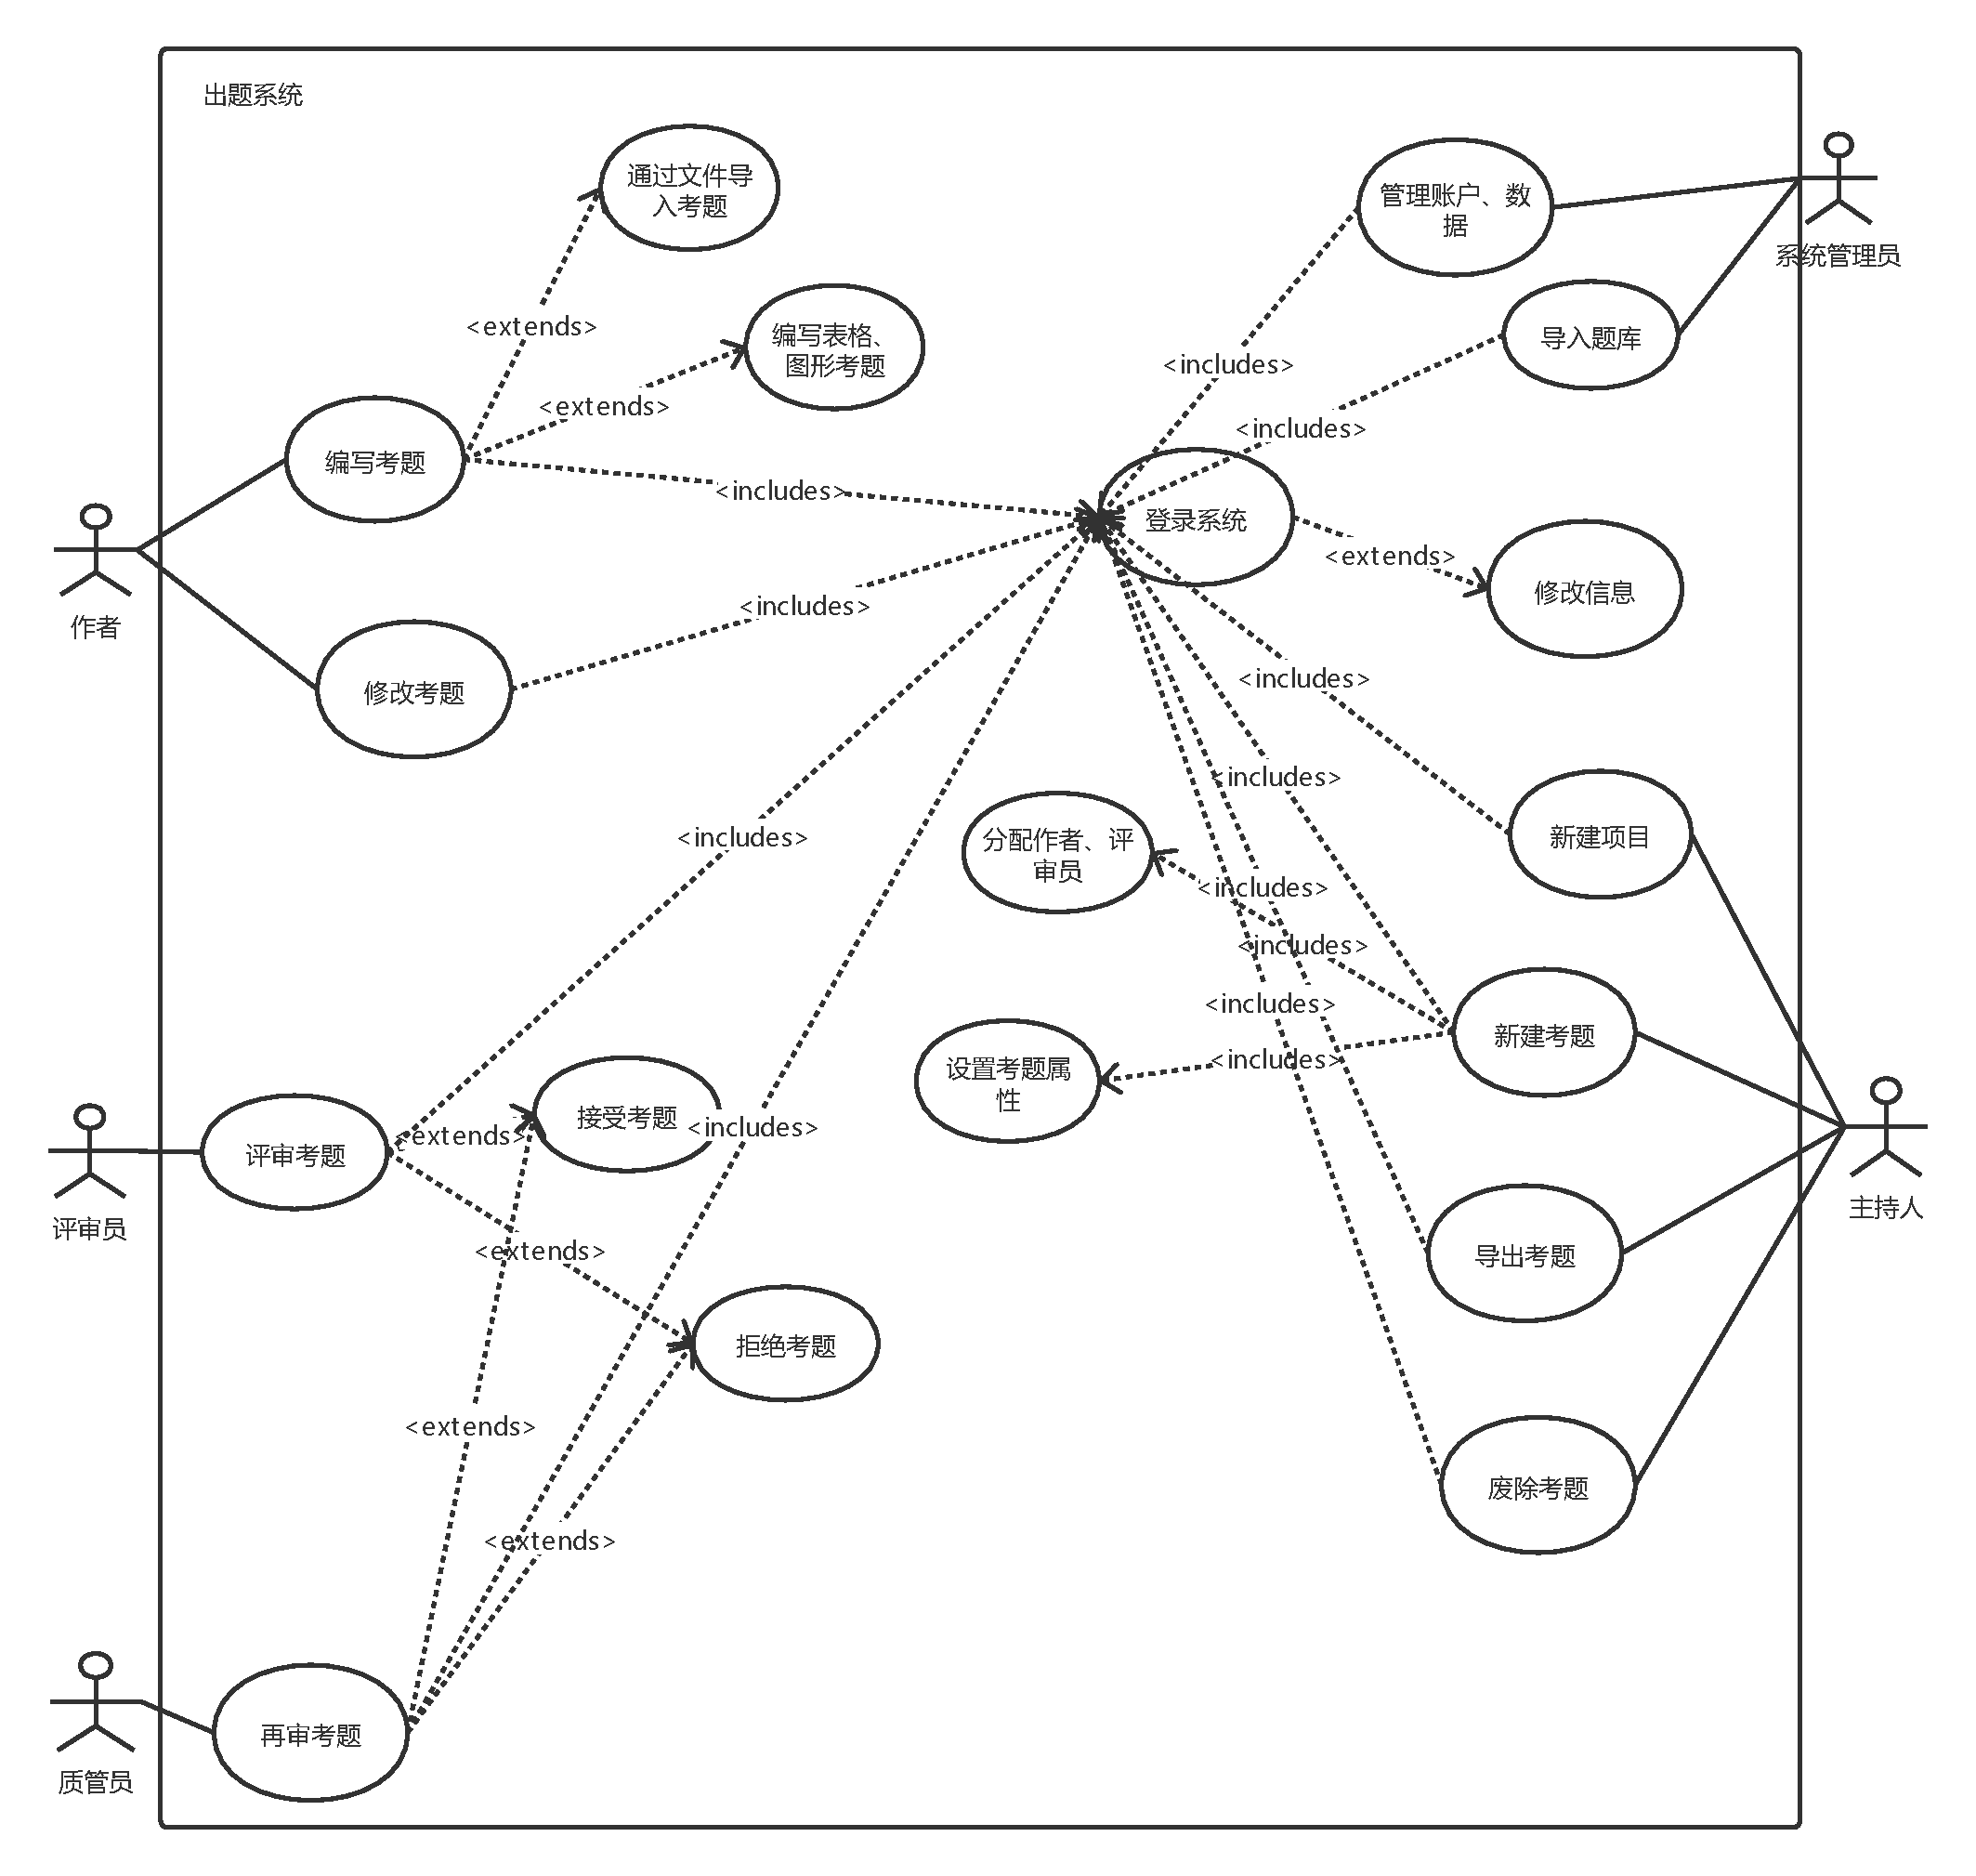
\includegraphics[scale=0.33]{./assets/usecase_diagram.pdf}
  \caption{整体用况图}\label{1}
\end{figure}

\begin{figure}
  \centering
  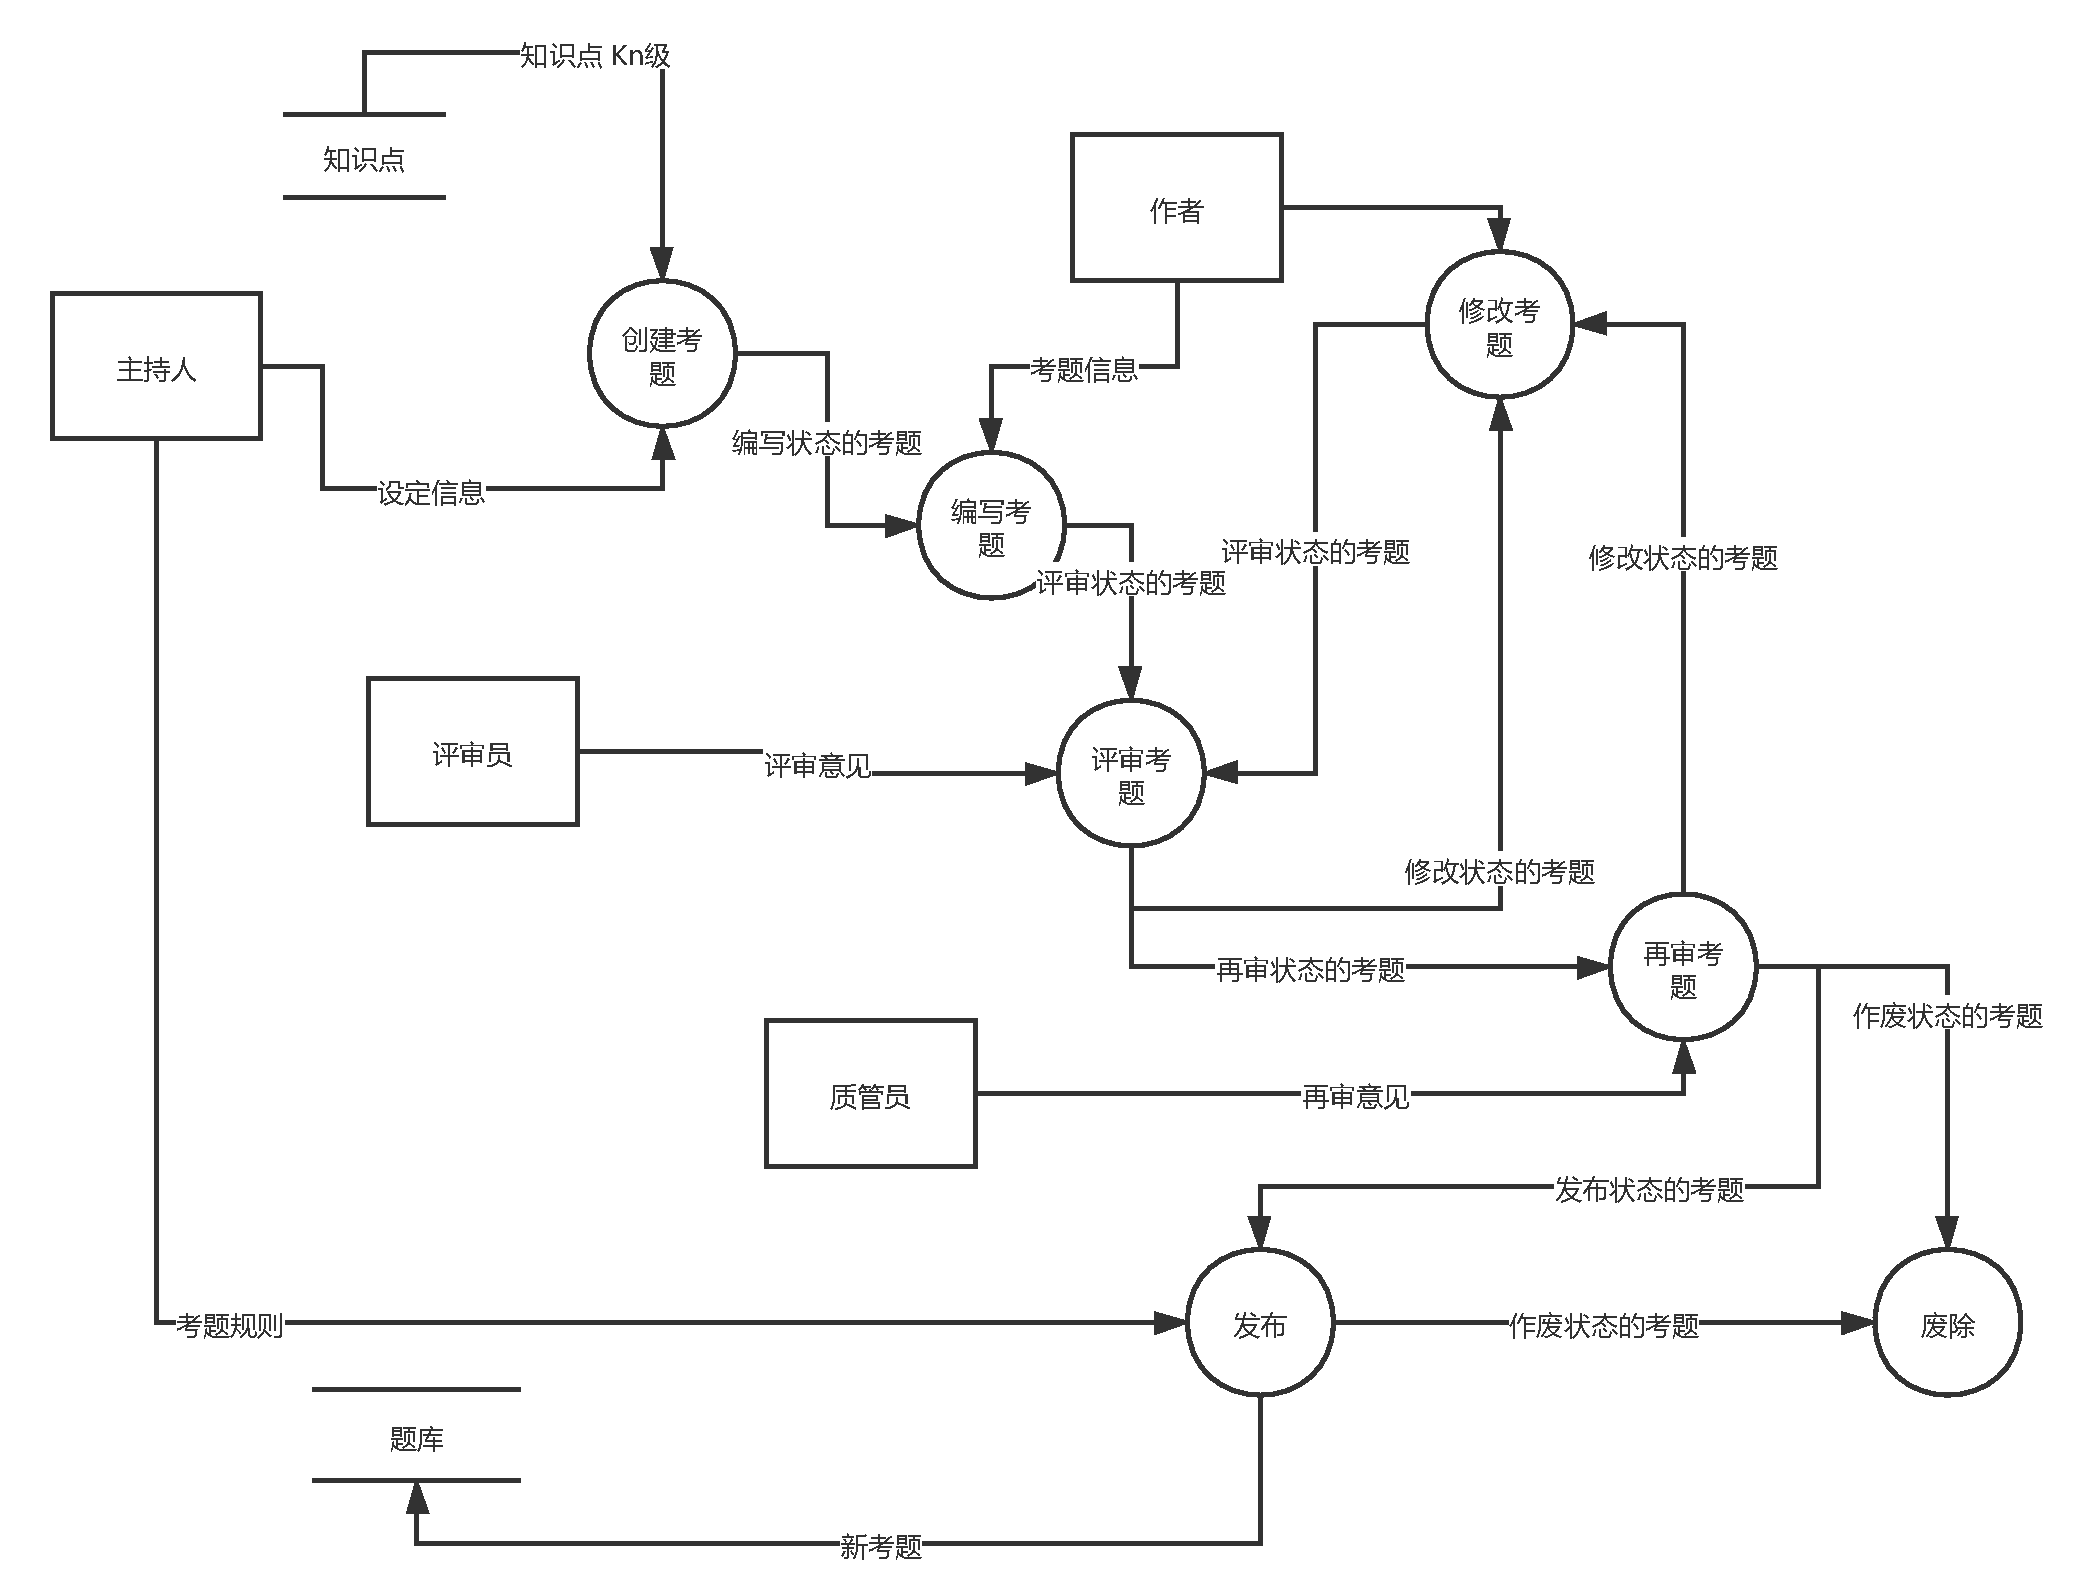
\includegraphics[scale=0.33]{./assets/dataflow_diagram.pdf}
  \caption{数据流图}\label{2}
\end{figure}

\begin{figure}
  \centering
  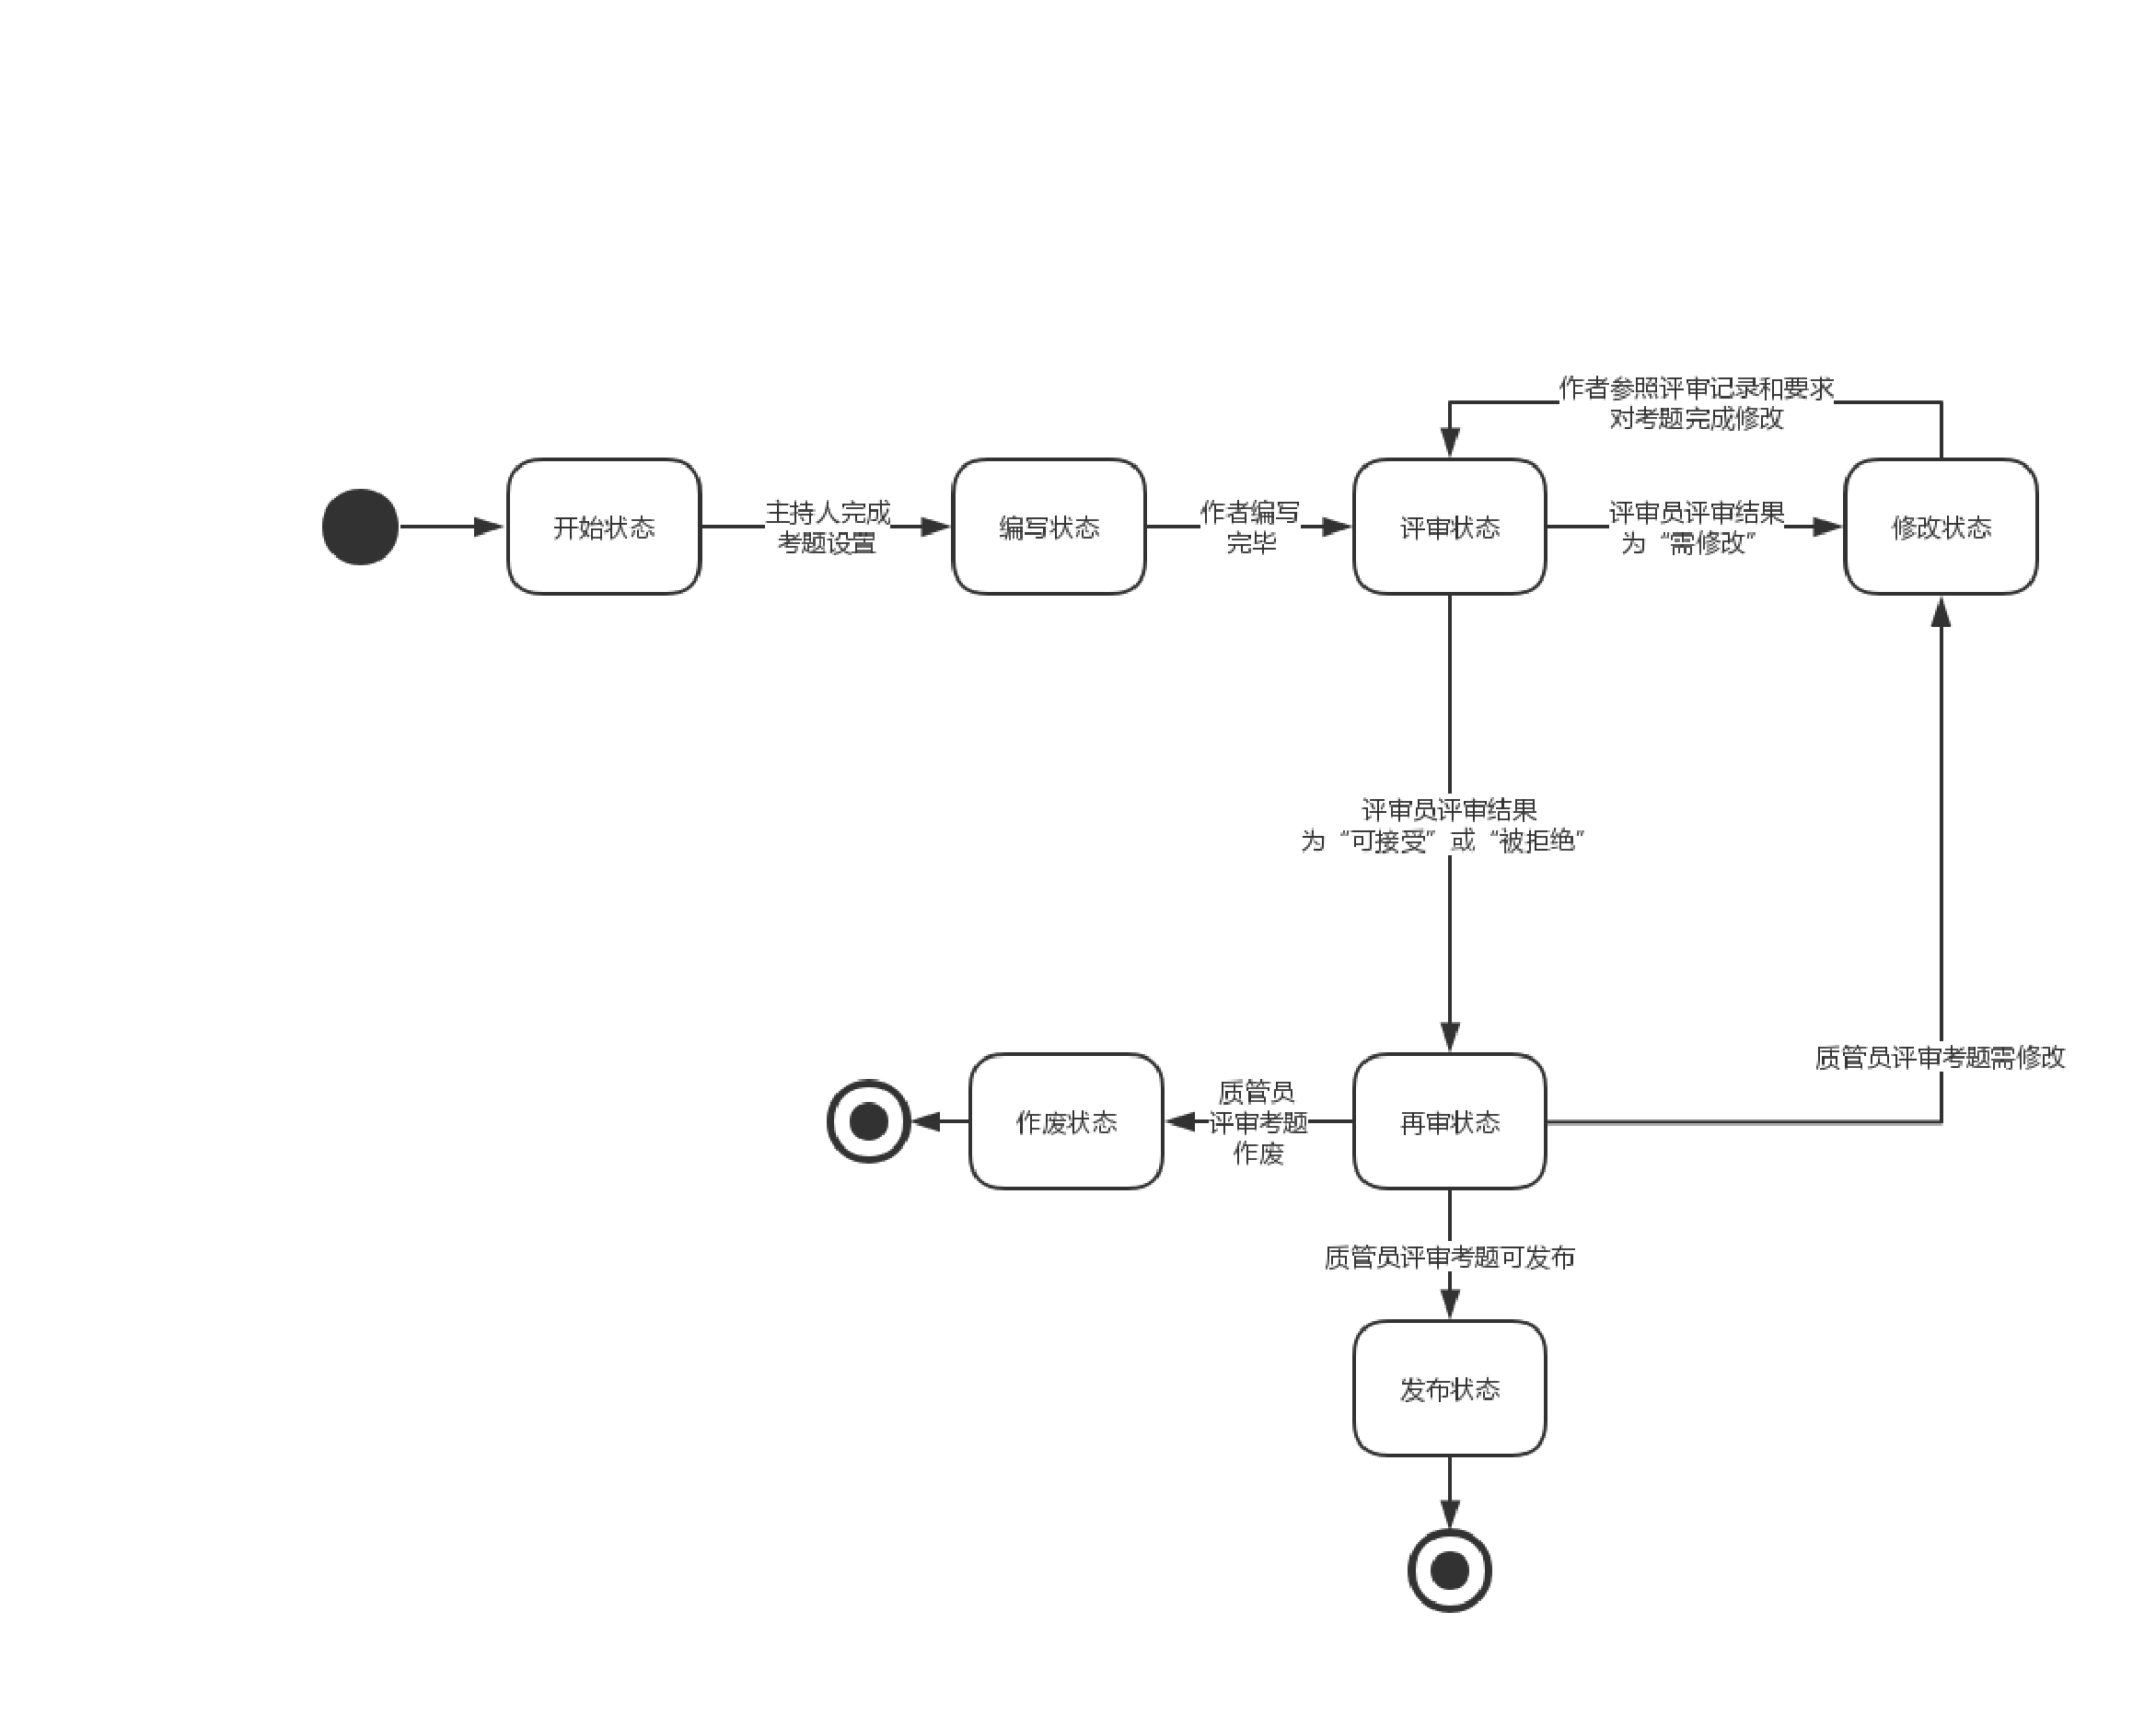
\includegraphics[scale=0.33]{./assets/status_diagram.pdf}
  \caption{状态机图}\label{3}
\end{figure}

\begin{figure}
  \centering
  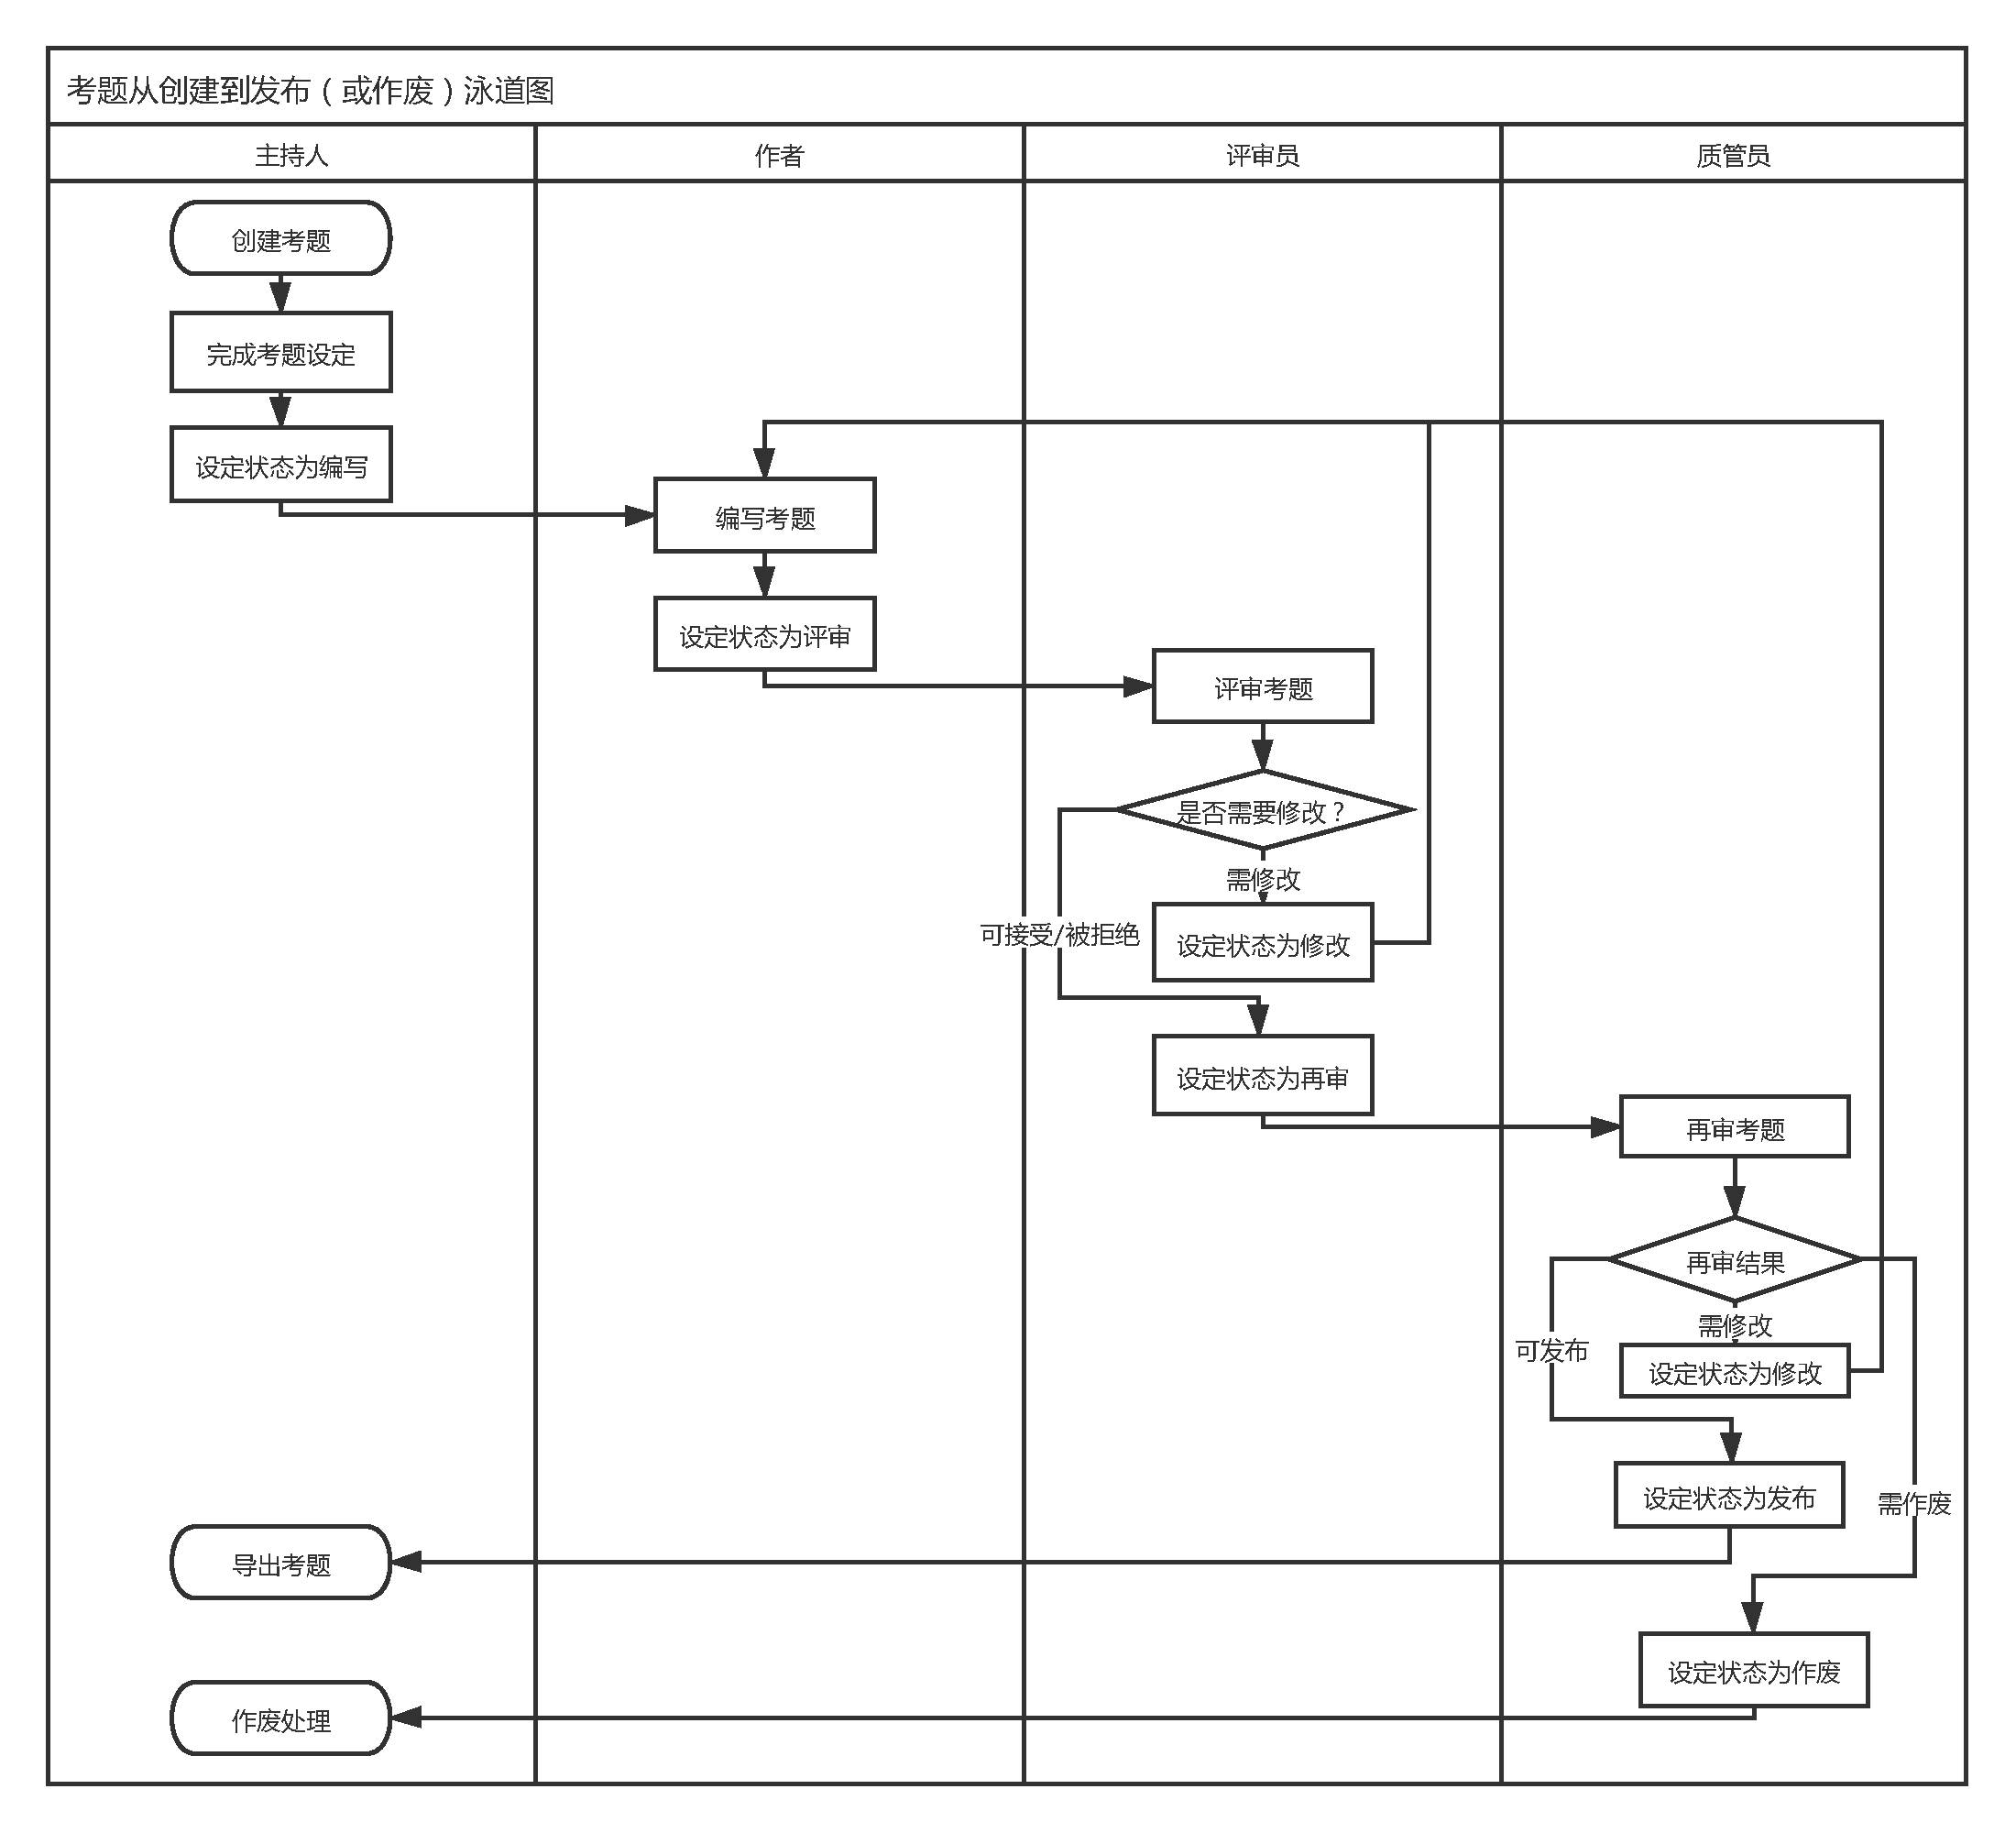
\includegraphics[scale=0.33]{./assets/swimlane_diagram.pdf}
  \caption{泳道图}\label{4}
\end{figure}

\pagebreak

\hypertarget{ux8d28ux91cfux9700ux6c42}{%
\section{质量需求}\label{ux8d28ux91cfux9700ux6c42}}

\hypertarget{ux54cdux5e94ux901fux5ea6}{%
\subsection{响应速度}\label{ux54cdux5e94ux901fux5ea6}}

\begin{itemize}
\tightlist
\item
  关键词:响应速度
\item
  需求描述:系统响应速度足够快,以避免打断用户的思路。
\item
  验收标准:在95\%的情况下,响应时间将不超过1.5秒,在其他情况下不超过4秒。
\end{itemize}

\hypertarget{ux5e76ux53d1ux8981ux6c42}{%
\subsection{并发要求}\label{ux5e76ux53d1ux8981ux6c42}}

\begin{itemize}
\tightlist
\item
  关键词:并发性
\item
  需求描述:出题系统要有协同工作的能力,能同时并行工作。
\item
  验收标准:支持动态用户(在线用户)在1500以上,支持静态用户(注册用户)在50000以上,支持并发数(同时工作用户)300以上。
\end{itemize}

\hypertarget{ux6d4fux89c8ux5668ux53efux79fbux690dux6027}{%
\subsection{浏览器可移植性}\label{ux6d4fux89c8ux5668ux53efux79fbux690dux6027}}

\begin{itemize}
\tightlist
\item
  关键词:浏览器兼容
\item
  需求描述:出题系统基于Web
  浏览器,可以在常见的和通用的浏览器的当前版本下正常工作。
\item
  验收标准:出题系统应在Internet Explorer,Firefox,google chrome,
  Opera最新版本下正常工作。
\end{itemize}

\hypertarget{ux5e73ux53f0ux53efux79fbux690dux6027}{%
\subsection{平台可移植性}\label{ux5e73ux53f0ux53efux79fbux690dux6027}}

\begin{itemize}
\tightlist
\item
  关键词:平台
\item
  需求描述:出题系统是不依赖与某种特定平台的系统。
\item
  验收标准:出题系统应可以正常运行在Windows 系统、Mac OS 或Linux 平台。
\end{itemize}

\hypertarget{ux6570ux636eux5e93ux53efux79fbux690dux6027}{%
\subsection{数据库可移植性}\label{ux6570ux636eux5e93ux53efux79fbux690dux6027}}

\begin{itemize}
\tightlist
\item
  关键词:数据库
\item
  需求描述:出题系统的数据库有很好的更新能力,能够适应迭代开发。
\item
  验收标准:至少支持免费的数据库系统(MySQL),替换关系数据库系统的平均时间不超过2小时,并且保证没有数据丢失。
\end{itemize}

\hypertarget{ux7528ux6237ux5b89ux5168ux6027ux9700ux6c42}{%
\subsection{用户安全性需求}\label{ux7528ux6237ux5b89ux5168ux6027ux9700ux6c42}}

\begin{itemize}
\tightlist
\item
  关键词:保密性~权限控制
\item
  需求描述:严格权限访问控制,用户在经过身份认证后,只能访问其权限范围内的数据,只能进行其权限范围内的操作。
\item
  验收标准:在1000次数据的修改全部由对应权限的人员完成,没有例外。
\end{itemize}

\hypertarget{ux7cfbux7edfux4e00ux81f4ux6027ux9700ux6c42}{%
\subsection{系统一致性需求}\label{ux7cfbux7edfux4e00ux81f4ux6027ux9700ux6c42}}

\begin{itemize}
\tightlist
\item
  关键词:断电~掉线~故障处理
\item
  需求描述:在断电、掉线情况下不会丢失数据。
\item
  验收标准:在1000次断电、掉线测试中数据保存完好,没有例外。
\end{itemize}

\hypertarget{ux6570ux636eux5b89ux5168ux6027ux9700ux6c42}{%
\subsection{数据安全性需求}\label{ux6570ux636eux5b89ux5168ux6027ux9700ux6c42}}

\begin{itemize}
\tightlist
\item
  关键词:数据安全
\item
  需求描述:系统必须保障数据安全。
\item
  验收标准:对一些重要的数据利用可靠的加密技术进行加密,例如用户的密码等。网络传递数据也应经过加密。需要保证数据在采集、传输和处理过程中不被偷窥、窃取、篡改。考题数据需要在存储时进行加密,确保不可破解。
\end{itemize}

\hypertarget{ux7cfbux7edfux5b89ux5168ux6027ux9700ux6c42}{%
\subsection{系统安全性需求}\label{ux7cfbux7edfux5b89ux5168ux6027ux9700ux6c42}}

\begin{itemize}
\tightlist
\item
  关键词:攻击
\item
  需求描述:必须保障系统的安全和可靠,具有防黑客能力,能经受来自互联网的一般性恶意攻击。
\item
  验收标准:能防止一般的病毒(包括木马)攻击、口令猜测攻击、黑客入侵等。至少99\%的攻击需要在10秒内检测到。
\end{itemize}

\hypertarget{ux6570ux636eux53efux9760ux6027}{%
\subsection{数据可靠性}\label{ux6570ux636eux53efux9760ux6027}}

\begin{itemize}
\tightlist
\item
  关键词:数据备份
\item
  需求描述:系统应保障出现故障后数据依旧完整。
\item
  验收标准:系统提供数据备份和恢复功能,使得在由于系统的错误或其他原因引起系统的数据丢失或系统的数据被破坏时,其中99\%的情况能够及时恢复和还原数据。
\end{itemize}

\hypertarget{ux7cfbux7edfux53efux9760ux6027}{%
\subsection{系统可靠性}\label{ux7cfbux7edfux53efux9760ux6027}}

\begin{itemize}
\tightlist
\item
  关键词:容错性~健壮性
\item
  需求描述:系统具有一定的容错和抗干扰能力,能处理系统运行过程中出现的各种异常情况,如:人为操作错误、输入非法数据、硬件设备失败等。
\item
  验收标准:在非硬件故障或非通讯故障时,系统能够保证正常运行,并有足够的提示信息帮助用户有效正确地完成任务。在10,000次错误测试中,因软件系统的失效而造成不能完成业务的概率小于5‰,最多出现1次需要重新启动系统的情况。
\end{itemize}

\hypertarget{ux7528ux6237ux6613ux7528ux6027}{%
\subsection{用户易用性}\label{ux7528ux6237ux6613ux7528ux6027}}

\begin{itemize}
\tightlist
\item
  关键词:易学习性~易理解性
\item
  需求描述:支持没有计算机使用经验、计算机使用经验较少及有较多计算机使用经验的用户方便地使用本系统。
\item
  验收标准:界面简洁美观,操作简单,80\%的用户在接受一个2小时的系统介绍培训后,可以熟练使用该系统。
\end{itemize}

\hypertarget{ux7cfbux7edfux6613ux7528ux6027}{%
\subsection{系统易用性}\label{ux7cfbux7edfux6613ux7528ux6027}}

\begin{itemize}
\tightlist
\item
  关键词:易操作性
\item
  需求描述:系统进行操作时有统一规范的提示信息。
\item
  验收标准:对必填项进行有效统一的提示;删除操作时,系统提示警示框,用户点击确认后,系统才执行删除操作,删除后可直接返回相关页面。
\end{itemize}

\hypertarget{ux5f00ux53d1ux4ebaux5458ux53efux7ef4ux62a4ux6027}{%
\subsection{开发人员可维护性}\label{ux5f00ux53d1ux4ebaux5458ux53efux7ef4ux62a4ux6027}}

\begin{itemize}
\tightlist
\item
  关键词:易分析性
\item
  需求描述:系统代码应便于开发人员维护。
\item
  验收标准:提供运行日志管理及安全审计功能,可追踪系统的历史使用情况,日志记录系统运行所发生的所有错误,包括本机错误和网络错误。保留系统对应的版本的源代码。代码有注释并且描述清晰。系统具有清晰的系统结构和命名规范,界面规范,提示和帮助信息规范,友好的错误提示信息,可以帮助用户自己找原因,自己维护系统。90\%的BUG修改时间不超过1个工作日,其他不超过2个工作日。
\end{itemize}

\hypertarget{ux7ea6ux675fux6761ux4ef6}{%
\section{约束条件}\label{ux7ea6ux675fux6761ux4ef6}}

\hypertarget{ux56fdux5bb6ux5b89ux5168ux6807ux51c6}{%
\subsection{国家安全标准}\label{ux56fdux5bb6ux5b89ux5168ux6807ux51c6}}

\begin{itemize}
\tightlist
\item
  关键词:国家安全标准
\item
  需求描述:系统安全性符合中华人民共和国国家标准GB/T 22239-2008。
\item
  验收标准:《信息系统安全等级保护基本要求》中每一项出题系统都符合。
\end{itemize}

\hypertarget{ux7f51ux7ad9ux4fe1ux606fux670dux52a1ux6807ux51c6}{%
\subsection{网站信息服务标准}\label{ux7f51ux7ad9ux4fe1ux606fux670dux52a1ux6807ux51c6}}

\begin{itemize}
\tightlist
\item
  关键词:信息服务标准
\item
  需求描述:系统运营符合《非经营性互联网信息服务备案管理办法》。
\item
  验收标准:做好已备案网站主页备案编号的悬挂和链接工作。
\end{itemize}

\hypertarget{ux91cdux6784ux9700ux6c42ux8bf4ux660e}{%
\section{重构需求说明}\label{ux91cdux6784ux9700ux6c42ux8bf4ux660e}}

\hypertarget{ux8bc4ux5ba1ux5458ux6807ux6ce8ux62d2ux7eddux7684ux9898ux76eeux53efux88abux8d28ux7ba1ux5458ux91cdux65b0ux5207ux6362ux4e3aux4feeux6539}{%
\subsection{评审员标注``拒绝''的题目可被质管员重新切换为修改}\label{ux8bc4ux5ba1ux5458ux6807ux6ce8ux62d2ux7eddux7684ux9898ux76eeux53efux88abux8d28ux7ba1ux5458ux91cdux65b0ux5207ux6362ux4e3aux4feeux6539}}

\begin{itemize}
\tightlist
\item
  对应需求:2.6.1 再审需修改
\item
  修改后的需求:关于考题再审,前一版需求文档中对于评审员``拒绝'',但质管员认为``还可''的考题处理情况没有进行说明。这里补充的是,当质管员认为题目仍然可以使用时,可将``被拒绝''的题目状态改为``修改'',并邮件通知作者。
\item
  对应的不合理需求:原版需求文档中,只提及了评审员``拒绝''的题目在后续审核中被质管员``废除'',我们认为无论是评审员``接受''或``拒绝''的题目在质管员处都可以在审核后改变为``发布''/``作废''/``修改''状态。
\end{itemize}

\hypertarget{ux5bf9ux8003ux9898ux5bfcux51faux89c4ux5219ux548cux5185ux5bb9ux4f5cux51faux9650ux5b9a}{%
\subsection{对考题导出规则和内容作出限定}\label{ux5bf9ux8003ux9898ux5bfcux51faux89c4ux5219ux548cux5185ux5bb9ux4f5cux51faux9650ux5b9a}}

\begin{itemize}
\tightlist
\item
  对应需求:2.8.1 导出发布考题
\item
  补充了前一版需求文档中对于考题导出规则和内容的限定的缺失,使得需求更加完善明确。
\end{itemize}

\pagebreak

\hypertarget{ux53c2ux8003ux6587ux732e}{%
\section*{参考文献}\label{ux53c2ux8003ux6587ux732e}}
\addcontentsline{toc}{section}{参考文献}

\hypertarget{refs}{}
\leavevmode\hypertarget{ref-innovativeInternationalisation}{}%
International Organization for Standardization. 2014. \emph{Systems and
Software Engineering --- Systems and Software Quality Requirements and
Evaluation (SQuaRE) --- Guide to SQuaRE}. \emph{International
Organization for Standardization}. Vol. 2014.
\url{https://www.iso.org/standard/64764.html}.

\leavevmode\hypertarget{ref-innovative1}{}%
中国国家标准化管理委员会. 2016. \emph{GB/T
25000.51-2016《系统与软件工程系统与软件质量要求和评价 (SQuaRE) 第 51
部分 : 就绪可用软件产品 (RUSP) 的质量要求和测试细则》}.
\emph{系统与软件工程系统与软件质量要求和评价 (SQuaRE)}. Vol. 51.
中国国家标准化管理委员会. \url{http://openstd.samr.gov.cn}.

\leavevmode\hypertarget{ref-innovative3}{}%
---------. 2017a. \emph{GB/T 25000.12-2017《系统与软件工程
系统与软件质量要求和评价(SQuaRE) 第12部分:数据质量模型》}.
\emph{系统与软件工程系统与软件质量要求和评价 (SQuaRE)}. Vol. 12.
中国国家标准化管理委员会. \url{http://openstd.samr.gov.cn}.

\leavevmode\hypertarget{ref-innovative4}{}%
---------. 2017b. \emph{GB/T 25000.24-2017《系统与软件工程
系统与软件质量要求和评价(SQuaRE) 第24部分:数据质量测量》}.
\emph{系统与软件工程系统与软件质量要求和评价 (SQuaRE)}. Vol. 24.
中国国家标准化管理委员会. \url{http://openstd.samr.gov.cn}.

\leavevmode\hypertarget{ref-innovative5}{}%
---------. 2018. \emph{GB/T 25000.40-201《系统与软件工程
系统与软件质量要求和评价(SQuaRE) 第40部分:评价过程》}.
\emph{系统与软件工程系统与软件质量要求和评价 (SQuaRE)}. Vol. 40.
中国国家标准化管理委员会. \url{http://openstd.samr.gov.cn}.

\leavevmode\hypertarget{ref-innovative2}{}%
---------. 2019. \emph{GB/T 25000.23-2019《系统与软件工程
系统与软件质量要求和评价(SQuaRE) 第23部分:系统与软件产品质量测量》}.
\emph{系统与软件工程系统与软件质量要求和评价 (SQuaRE)}. Vol. 23.
中国国家标准化管理委员会. \url{http://openstd.samr.gov.cn}.

\end{document}
